\documentclass[tikz,border=2pt]{standalone}
\usepackage{amsmath}
\begin{document}
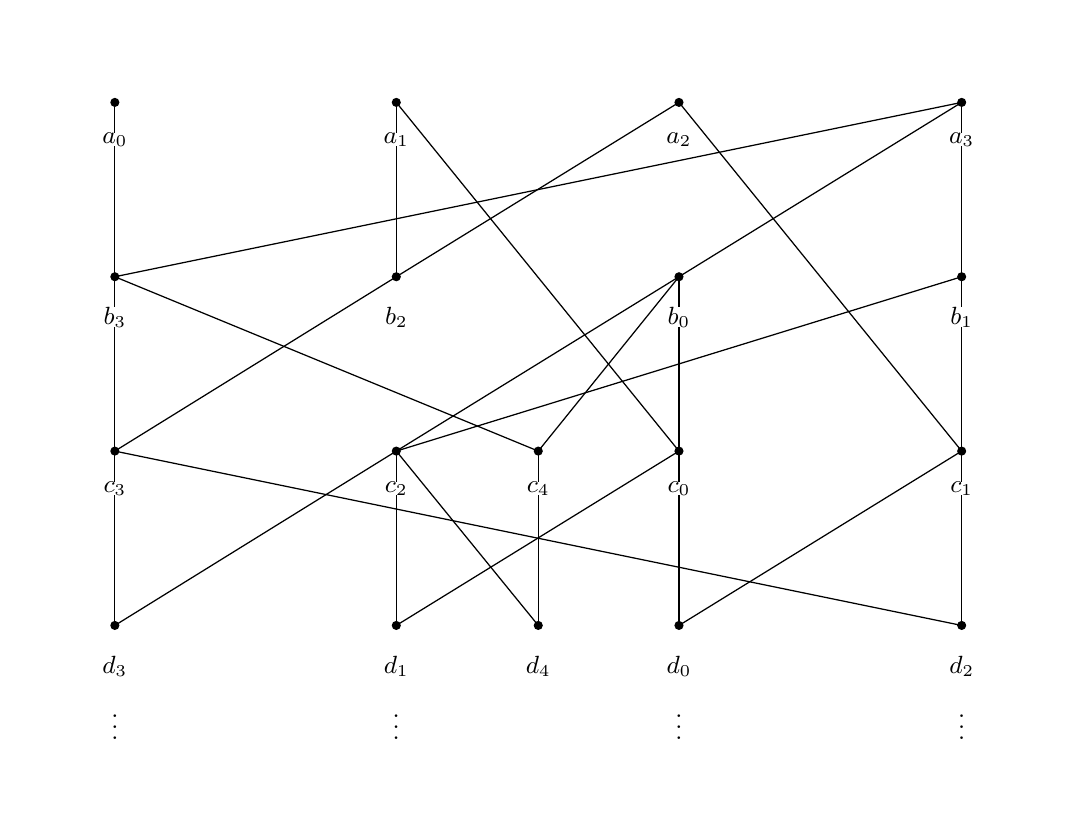
\begin{tikzpicture}[x=.45pt,y=-.45pt,line width=.45pt,line cap=round,font=\fontsize{9}{10}\selectfont]
\path[use as bounding box] (90,30) rectangle (910,655);
\coordinate (na0) at (160,90);
\coordinate (na1) at (386,90);
\coordinate (na2) at (613,90);
\coordinate (na3) at (840,90);
\coordinate (nb0) at (613,230);
\coordinate (nb1) at (840,230);
\coordinate (nb2) at (386,230);
\coordinate (nb3) at (160,230);
\coordinate (nc0) at (613,370);
\coordinate (nc1) at (840,370);
\coordinate (nc2) at (386,370);
\coordinate (nc3) at (160,370);
\coordinate (nc4) at (500,370);
\coordinate (nd0) at (613,510);
\coordinate (nd1) at (386,510);
\coordinate (nd2) at (840,510);
\coordinate (nd3) at (160,510);
\coordinate (nd4) at (500,510);
\draw (nb0) -- (na3);
\draw (nb1) -- (na3);
\draw (nb2) -- (na1);
\draw (nb2) -- (na2);
\draw (nb3) -- (na0);
\draw (nb3) -- (na3);
\draw (nc0) -- (nb0);
\draw (nc0) -- (na1);
\draw (nc1) -- (nb1);
\draw (nc1) -- (na2);
\draw (nc2) -- (nb0);
\draw (nc2) -- (nb1);
\draw (nc3) -- (nb2);
\draw (nc3) -- (nb3);
\draw (nc4) -- (nb0);
\draw (nc4) -- (nb3);
\draw (nd0) -- (nc0);
\draw (nd0) -- (nc1);
\draw (nd1) -- (nc0);
\draw (nd1) -- (nc2);
\draw (nd2) -- (nc1);
\draw (nd2) -- (nc3);
\draw (nd3) -- (nc2);
\draw (nd3) -- (nc3);
\draw (nd4) -- (nc2);
\draw (nd4) -- (nc4);
\node at (160,585) {$\vdots$};
\node at (386,585) {$\vdots$};
\node at (613,585) {$\vdots$};
\node at (840,585) {$\vdots$};
\fill (na0) circle[radius=1.65pt];
\node[anchor=north,inner sep=0pt,fill=white] at (160,114) {$a_{0}$};
\fill (na1) circle[radius=1.65pt];
\node[anchor=north,inner sep=0pt,fill=white] at (386,114) {$a_{1}$};
\fill (na2) circle[radius=1.65pt];
\node[anchor=north,inner sep=0pt,fill=white] at (613,114) {$a_{2}$};
\fill (na3) circle[radius=1.65pt];
\node[anchor=north,inner sep=0pt,fill=white] at (840,114) {$a_{3}$};
\fill (nb0) circle[radius=1.65pt];
\node[anchor=north,inner sep=0pt,fill=white] at (613,254) {$b_{0}$};
\fill (nb1) circle[radius=1.65pt];
\node[anchor=north,inner sep=0pt,fill=white] at (840,254) {$b_{1}$};
\fill (nb2) circle[radius=1.65pt];
\node[anchor=north,inner sep=0pt,fill=white] at (386,254) {$b_{2}$};
\fill (nb3) circle[radius=1.65pt];
\node[anchor=north,inner sep=0pt,fill=white] at (160,254) {$b_{3}$};
\fill (nc0) circle[radius=1.65pt];
\node[anchor=north,inner sep=0pt,fill=white] at (613,394) {$c_{0}$};
\fill (nc1) circle[radius=1.65pt];
\node[anchor=north,inner sep=0pt,fill=white] at (840,394) {$c_{1}$};
\fill (nc2) circle[radius=1.65pt];
\node[anchor=north,inner sep=0pt,fill=white] at (386,394) {$c_{2}$};
\fill (nc3) circle[radius=1.65pt];
\node[anchor=north,inner sep=0pt,fill=white] at (160,394) {$c_{3}$};
\fill (nc4) circle[radius=1.65pt];
\node[anchor=north,inner sep=0pt,fill=white] at (500,394) {$c_{4}$};
\fill (nd0) circle[radius=1.65pt];
\node[anchor=north,inner sep=0pt,fill=white] at (613,534) {$d_{0}$};
\fill (nd1) circle[radius=1.65pt];
\node[anchor=north,inner sep=0pt,fill=white] at (386,534) {$d_{1}$};
\fill (nd2) circle[radius=1.65pt];
\node[anchor=north,inner sep=0pt,fill=white] at (840,534) {$d_{2}$};
\fill (nd3) circle[radius=1.65pt];
\node[anchor=north,inner sep=0pt,fill=white] at (160,534) {$d_{3}$};
\fill (nd4) circle[radius=1.65pt];
\node[anchor=north,inner sep=0pt,fill=white] at (500,534) {$d_{4}$};
\end{tikzpicture}
\end{document}
